\documentclass[a4paper,12pt]{report}
\usepackage[utf8]{inputenc}
\usepackage[T5]{fontenc}
\usepackage{lmodern}
\usepackage[vietnamese]{babel}
\usepackage{amsmath}
\usepackage{graphicx}
\usepackage{hyperref}
\usepackage{float}
\usepackage{booktabs}
\usepackage{geometry}
\usepackage{listings}
\usepackage{xcolor}
\usepackage{longtable}
\usepackage{tabularx}
\usepackage{array}
\usepackage{caption}
\usepackage{subcaption}
\usepackage{url}
\usepackage{setspace}
\usepackage{microtype}
\usepackage{enumitem}

% Fix spacing and overflow issues (Overfull/Underfull \hbox)
\tolerance=1000
\emergencystretch=3em
\clubpenalty=10000
\widowpenalty=10000

\graphicspath{{../uml/}{../demo/}{./}}
\onehalfspacing

% Allow line breaks in \texttt
\renewcommand{\texttt}[1]{%
  \begingroup
  \ttfamily
  \hyphenchar\font=`\-
  #1%
  \endgroup
}

\geometry{
    a4paper,
    left=25mm,
    right=25mm,
    top=20mm,
    bottom=20mm,
}

\hypersetup{
    colorlinks=true,
    linkcolor=blue,
    urlcolor=blue,
    citecolor=blue
}

% Setup for code listings
\definecolor{codegreen}{rgb}{0,0.6,0}
\definecolor{codegray}{rgb}{0.5,0.5,0.5}
\definecolor{codepurple}{rgb}{0.58,0,0.82}
\definecolor{backcolour}{rgb}{0.95,0.95,0.92}

\lstdefinestyle{mystyle}{
    backgroundcolor=\color{backcolour},
    commentstyle=\color{codegreen},
    keywordstyle=\color{magenta},
    numberstyle=\tiny\color{codegray},
    stringstyle=\color{codepurple},
    basicstyle=\ttfamily\footnotesize,
    breakatwhitespace=false,
    breaklines=true,
    captionpos=b,
    keepspaces=true,
    numbers=left,
    numbersep=5pt,
    showspaces=false,
    showstringspaces=false,
    showtabs=false,
    tabsize=2
}

\lstset{style=mystyle, escapeinside={(*}{*)}}

% API path helper to allow clean line breaks in tables
\newcommand{\apipath}[1]{\begingroup\small\nolinkurl{#1}\endgroup}
% Inline code helper with safe line breaks (underscores, slashes)
\newcommand{\code}[1]{\begingroup\ttfamily\small\nolinkurl{#1}\endgroup}

\begin{document}

% =====================================================
% TRANG BÌA
% =====================================================
\begin{titlepage}
    \centering
    \vspace*{1cm}

    \Large \textbf{ĐẠI HỌC QUỐC GIA HÀ NỘI} \\
    \Large \textbf{TRƯỜNG ĐẠI HỌC CÔNG NGHỆ (UET)} \\
    \vspace{1.2cm}

    \Large \textbf{BÁO CÁO MÔN HỌC} \\
    \vspace{0.4cm}
    \huge \textbf{SMART ATTENDANCE SYSTEM} \\
    \Large \textbf{Hệ Thống Điểm Danh Thông Minh} \\
    \vspace{0.8cm}

    \begin{center}
        \textbf{Phiên bản:} \texttt{v1.0.3} \\
        \textbf{Ngày tạo:} \texttt{\today}
    \end{center}

    \vspace{1.0cm}

    \begin{flushleft}
        \Large
        \textbf{Giảng viên hướng dẫn:} \\
        \vspace{0.3cm}
        \begin{tabular*}{\textwidth}{@{\extracolsep{\fill}} c c c @{} }
            \Large Đào Việt Anh & \Large Lương Sơn Bá & \Large Trịnh Ngọc Huỳnh
        \end{tabular*}
        \vspace{0.8cm}

        \textbf{Nhóm sinh viên thực hiện (Nhóm 9):} \\
        \normalsize
        1. 24022454 Lê Việt Thành (Trưởng nhóm - DevOps Lead) \\
        2. 24022406 Nguyễn Nhật Minh (Backend Developer) \\
        3. 24022364 Tạ Duy Khánh (AI/ML Engineer) \\
        4. 24022394 Nguyễn Đức Mạnh (Frontend Developer) \\
    \end{flushleft}

    \vfill

    \Large Hà Nội, Tháng 05/2026
\end{titlepage}

\tableofcontents
\newpage

% =====================================================
% CHƯƠNG 1: GIỚI THIỆU ĐỀ TÀI
% =====================================================
\chapter{Giới thiệu đề tài}

\section{Bối cảnh và bài toán}
Chuyển đổi số trong giáo dục đòi hỏi các hệ thống quản lý học vụ phải chính xác, minh bạch và giảm tối đa thao tác thủ công. Các phương pháp điểm danh truyền thống (gọi tên, thẻ từ, vân tay) đều gặp hạn chế về thời gian, chi phí và khả năng gian lận. Dự án \textbf{Smart Attendance System} hướng tới một quy trình điểm danh tự động hóa bằng nhận diện khuôn mặt, bảo đảm xác minh đúng danh tính theo mã sinh viên.

\section{Mục tiêu}
\begin{itemize}[leftmargin=*]
    \item \textbf{Xác minh 1-1 theo mã sinh viên}: hạn chế nhầm lẫn và loại bỏ điểm danh hộ.
    \item \textbf{Tối ưu thời gian}: giảm thời gian điểm danh xuống mức giây cho mỗi lượt.
    \item \textbf{Kiến trúc mở rộng}: tách luồng AI ra khỏi API bằng Celery/Redis để xử lý đồng thời nhiều yêu cầu.
    \item \textbf{Quản trị rõ ràng}: hỗ trợ duyệt sinh viên, duyệt lịch học, sửa trạng thái điểm danh, xuất báo cáo.
\end{itemize}

\section{Phạm vi và đối tượng sử dụng}
Hệ thống xử lý hai luồng nghiệp vụ chính: \textit{Đăng ký hồ sơ sinh viên} và \textit{Điểm danh \& Quản trị}.

\begin{table}[H]
\centering
\begin{tabularx}{\textwidth}{|l|X|X|}
\hline
\textbf{Đối tượng} & \textbf{Nghiệp vụ cốt lõi} & \textbf{Quyền hạn tương tác} \\ \hline
\textbf{Sinh viên} & Đăng ký khuôn mặt, đăng ký lịch học & Gửi ảnh/video đăng ký, cập nhật lịch học, điểm danh check-in/check-out. \\ \hline
\textbf{Giảng viên/Admin} & Duyệt sinh viên, duyệt lịch học, quản trị điểm danh & Xem thống kê, nhật ký, sửa trạng thái, xuất CSV. \\ \hline
\end{tabularx}
\caption{Đối tượng sử dụng và phạm vi nghiệp vụ}
\end{table}

% =====================================================
% CHƯƠNG 2: THÀNH VIÊN VÀ PHÂN CÔNG NHIỆM VỤ
% =====================================================
\chapter{Thành viên và phân công nhiệm vụ}

\section{Danh sách thành viên}
Bảng \ref{tab:thanhvien} trình bày thông tin các thành viên trong nhóm, vai trò chính và tỉ lệ đóng góp vào dự án.

\begin{table}[H]
\centering
\begin{tabularx}{\textwidth}{|c|c|X|l|c|}
\hline
\textbf{STT} & \textbf{MSSV} & \textbf{Họ và tên} & \textbf{Vai trò chính} & \textbf{Đóng góp} \\ \hline
1 & 24022454 & Lê Việt Thành & Trưởng nhóm, DevOps & 25\% \\ \hline
2 & 24022406 & Nguyễn Nhật Minh & Backend Developer & 25\% \\ \hline
3 & 24022364 & Tạ Duy Khánh & AI/Worker Developer & 25\% \\ \hline
4 & 24022394 & Nguyễn Đức Mạnh & Frontend Developer & 25\% \\ \hline
\end{tabularx}
\caption{Thông tin thành viên và tỉ lệ đóng góp}
\label{tab:thanhvien}
\end{table}

\section{Phân công nhiệm vụ chi tiết}
Bảng \ref{tab:phancong} mô tả chi tiết nhiệm vụ được giao cho từng thành viên trong suốt quá trình phát triển dự án.

\begin{table}[H]
\centering
\begin{tabularx}{\textwidth}{|l|X|}
\hline
\textbf{Thành viên} & \textbf{Nhiệm vụ chi tiết} \\ \hline
Lê Việt Thành & Thiết kế kiến trúc hệ thống, cấu hình Docker Compose, thiết lập CI/CD pipeline, cấu hình Nginx reverse proxy, xây dựng Backup Service, triển khai hệ thống lên Internet (SSL + domain), viết tài liệu báo cáo. \\ \hline
Nguyễn Nhật Minh & Phát triển API FastAPI (Auth, Members, Schedule, Attendance, Dashboard), thiết kế database schema MySQL, xây dựng Scheduler/Cronjob quét vắng mặt, tích hợp xác thực JWT, xử lý logic điểm danh đa phiên. \\ \hline
Tạ Duy Khánh & Xây dựng Celery Worker, tích hợp DeepFace (ArcFace/RetinaFace), triển khai Qdrant Vector DB, phát triển pipeline trích xuất và so khớp vector khuôn mặt, cấu hình Redis cache cho embeddings. \\ \hline
Nguyễn Đức Mạnh & Phát triển giao diện Vue 3 SPA, xây dựng trang điểm danh sinh viên, dashboard quản trị, giao diện quản lý sinh viên và lịch học, thiết kế UI/UX, tích hợp API với frontend. \\ \hline
\end{tabularx}
\caption{Chi tiết nhiệm vụ của từng thành viên}
\label{tab:phancong}
\end{table}

% =====================================================
% CHƯƠNG 3: KIẾN TRÚC PHẦN MỀM
% =====================================================
\chapter{Kiến trúc phần mềm}

\section{Tổng quan kiến trúc}
Hệ thống Smart Attendance System được thiết kế theo kiến trúc \textbf{Microservices}, chia thành 5 tầng chính (Hình \ref{fig:sw_arch}):

\begin{enumerate}[leftmargin=*]
    \item \textbf{Presentation Layer} (Tầng trình diễn): Giao diện người dùng Vue 3 SPA được phục vụ qua Nginx reverse proxy, cung cấp các trang chức năng cho sinh viên (đăng ký, điểm danh) và giảng viên (dashboard, quản lý).
    \item \textbf{Application Layer} (Tầng nghiệp vụ): FastAPI backend xử lý toàn bộ logic nghiệp vụ bao gồm xác thực JWT, quản lý sinh viên, lịch học, điểm danh và thống kê. APScheduler chạy cronjob 23:59 hàng ngày để quét vắng mặt tự động.
    \item \textbf{AI Processing Layer} (Tầng xử lý AI): Celery Worker chạy nền, sử dụng DeepFace (mô hình ArcFace) để trích xuất vector khuôn mặt 512 chiều và RetinaFace để phát hiện khuôn mặt, thực hiện xác minh 1-1 với Qdrant Vector DB.
    \item \textbf{Data \& Storage Layer} (Tầng dữ liệu): Bao gồm MySQL 8.0 (dữ liệu quan hệ), Qdrant (vector embeddings), MinIO S3 (object storage cho ảnh), và Redis (message broker + cache).
    \item \textbf{Infrastructure Layer} (Tầng hạ tầng): Docker Compose đóng gói 8 container, CI/CD pipeline tự động build, và Backup Service sao lưu định kỳ.
\end{enumerate}

\begin{figure}[H]
    \centering
    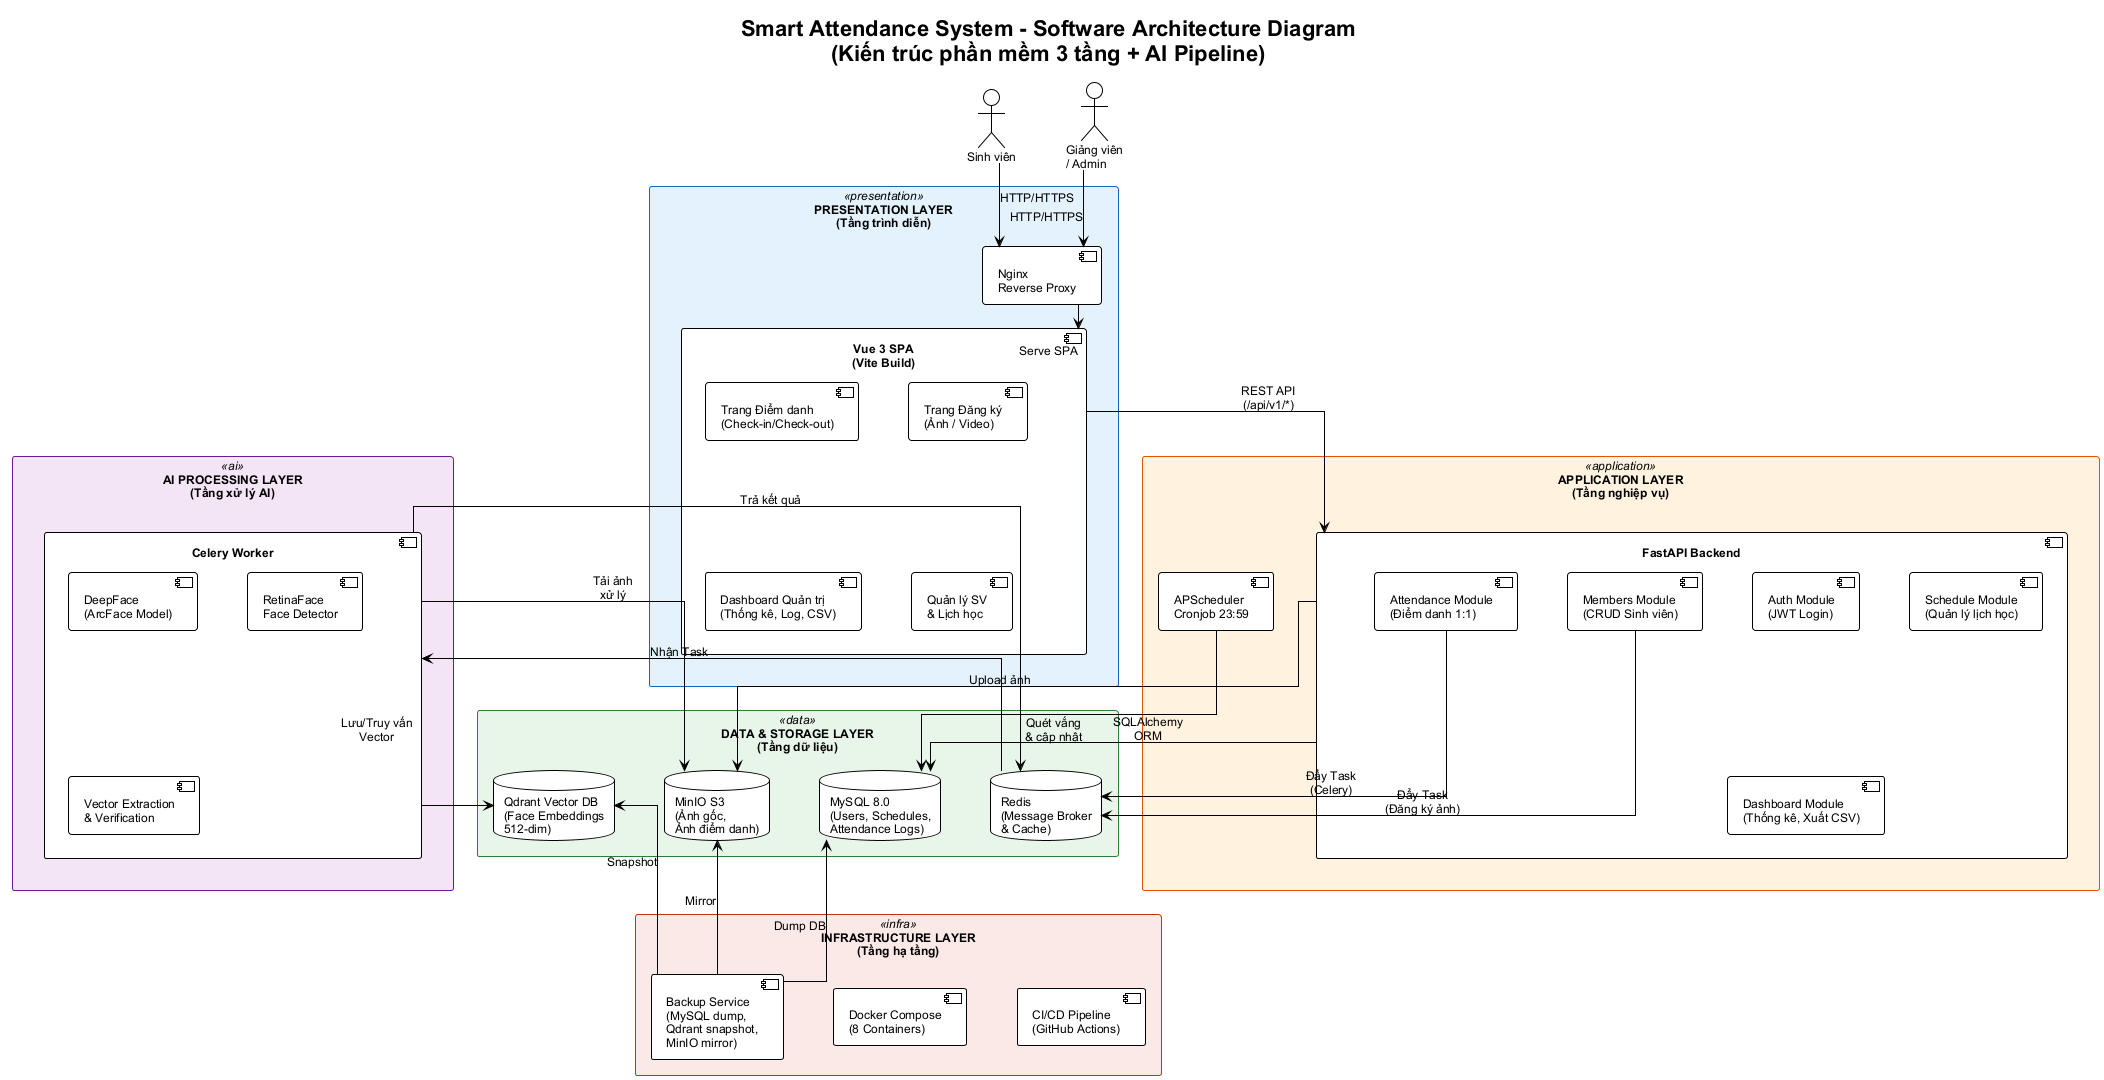
\includegraphics[width=0.95\textwidth]{software_architecture.png}
    \caption{Sơ đồ kiến trúc phần mềm (Software Architecture Diagram)}
    \label{fig:sw_arch}
\end{figure}

\section{Sơ đồ thành phần}
Sơ đồ thành phần (Hình \ref{fig:component}) chi tiết hóa các module bên trong mỗi tầng và luồng giao tiếp giữa chúng.

\begin{figure}[H]
    \centering
    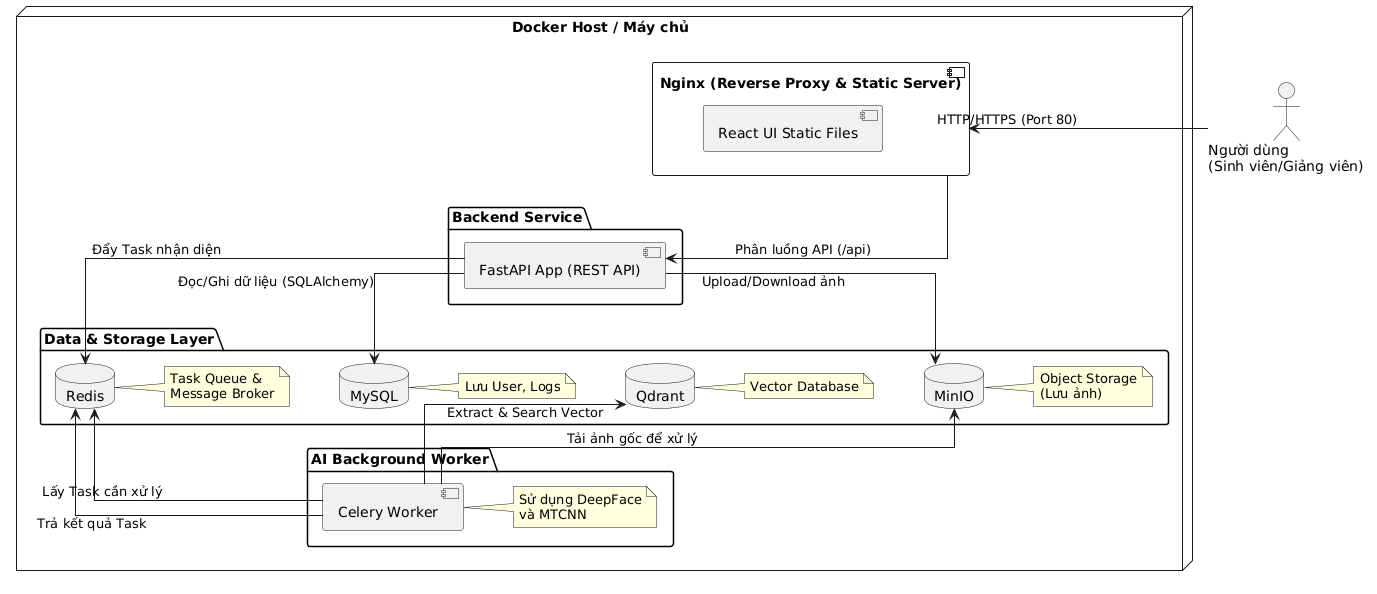
\includegraphics[width=0.95\textwidth]{component.png}
    \caption{Sơ đồ thành phần (Component Diagram)}
    \label{fig:component}
\end{figure}

\section{Sơ đồ triển khai}
Hệ thống triển khai trên Docker Host với 8 container kết nối qua bridge network \texttt{attendance\_net} (Hình \ref{fig:deployment}).

\begin{figure}[H]
    \centering
    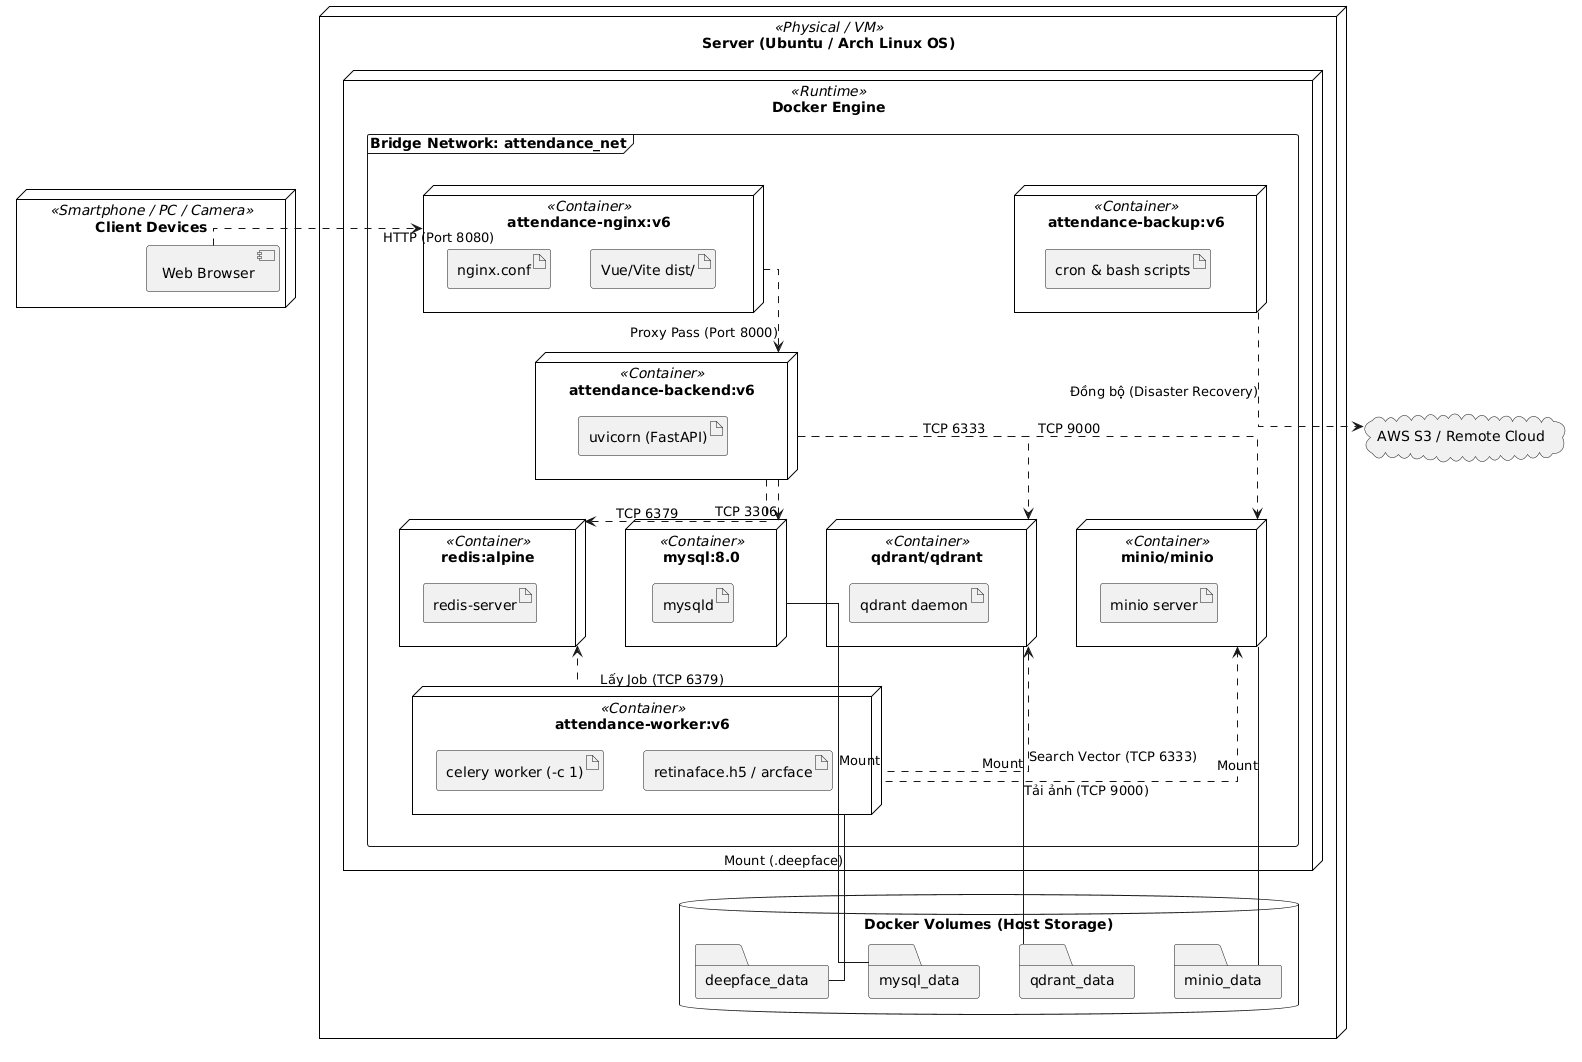
\includegraphics[width=0.95\textwidth]{deployment.png}
    \caption{Sơ đồ triển khai (Deployment Diagram) với Docker}
    \label{fig:deployment}
\end{figure}

\section{Công nghệ sử dụng}
\begin{table}[H]
\centering
\begin{tabularx}{\textwidth}{|l|X|X|}
\hline
\textbf{Tầng} & \textbf{Công nghệ} & \textbf{Vai trò} \\ \hline
Frontend & Vue 3 + Vite & Giao diện điểm danh và dashboard quản trị. \\ \hline
Backend & FastAPI + SQLAlchemy & API xử lý nghiệp vụ, auth, thống kê. \\ \hline
AI Worker & Celery + DeepFace & Trích xuất vector, so khớp khuôn mặt. \\ \hline
Vector DB & Qdrant & Lưu và truy vấn vector theo student\_id. \\ \hline
RDBMS & MySQL 8.0 & Lưu thông tin sinh viên, lịch học, log điểm danh. \\ \hline
Cache/Queue & Redis & Hàng đợi Celery và cache. \\ \hline
Object Storage & MinIO & Lưu ảnh gốc và ảnh điểm danh. \\ \hline
Gateway & Nginx & Reverse proxy cho frontend và API. \\ \hline
Deploy & Docker Compose & Đóng gói, triển khai nhanh toàn hệ thống. \\ \hline
\end{tabularx}
\caption{Bảng công nghệ chính của dự án}
\end{table}

\section{Luồng xử lý chính}
\begin{figure}[H]
    \centering
    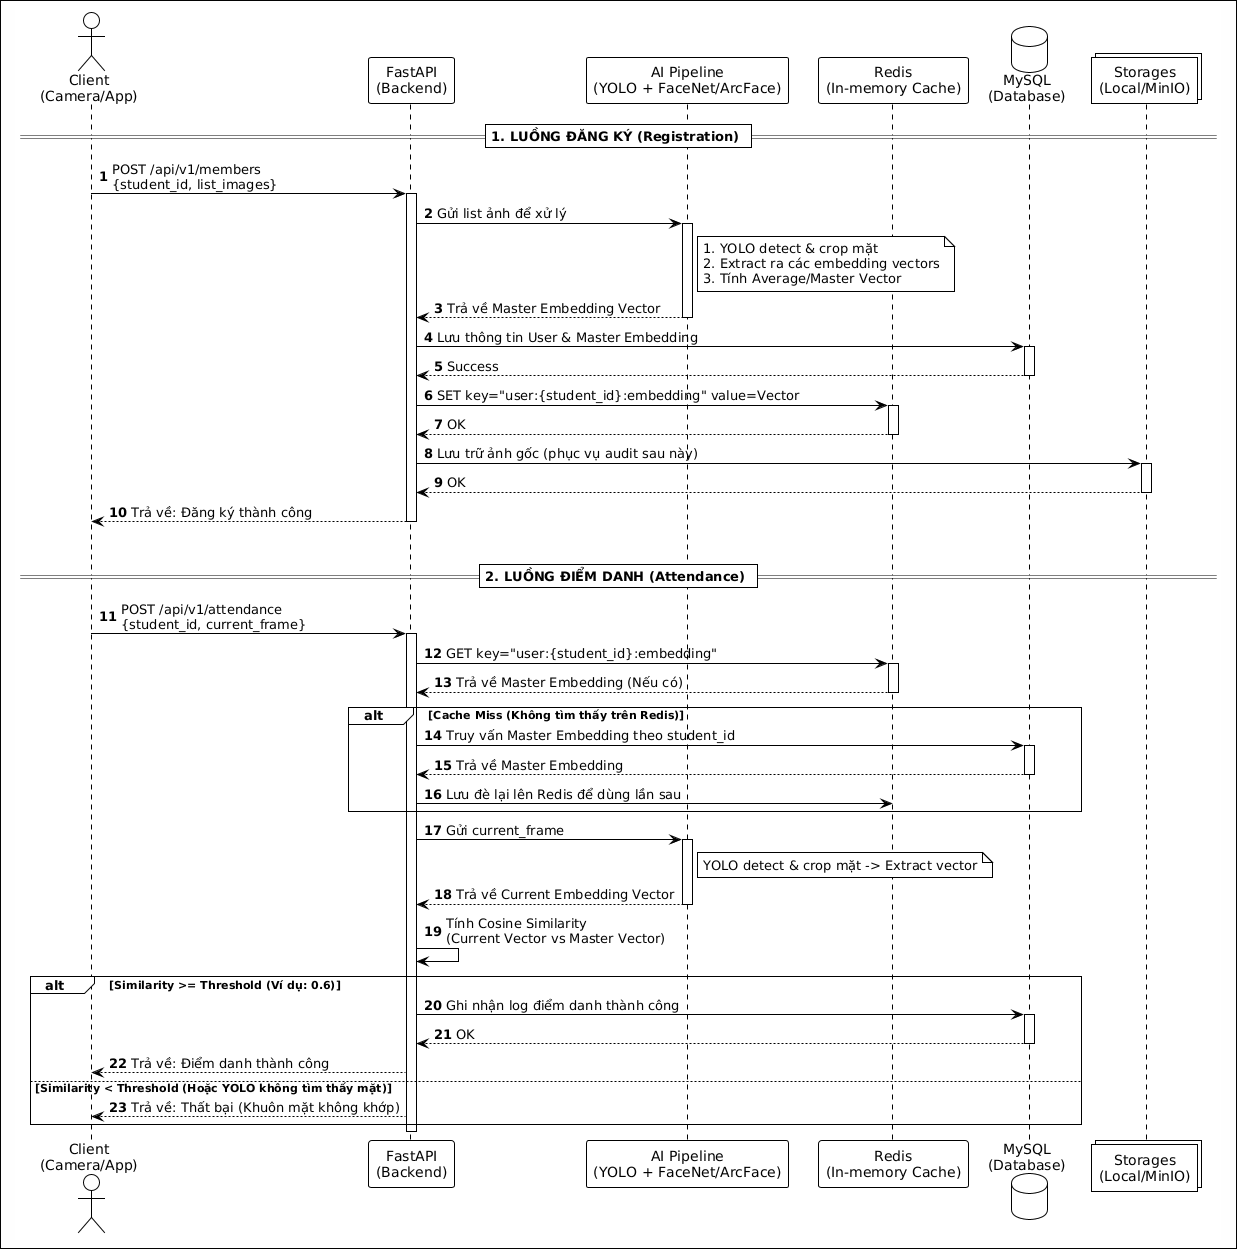
\includegraphics[width=0.90\textwidth,height=0.70\textheight,keepaspectratio]{sequency.png}
    \caption{Sơ đồ tuần tự cho luồng đăng ký/điểm danh}
    \label{fig:sequence}
\end{figure}

Hình \ref{fig:sequence} mô tả chuỗi xử lý chính: frontend gửi yêu cầu, backend kiểm tra dữ liệu và tải ảnh lên MinIO, sau đó đẩy tác vụ vào Redis để worker trích xuất vector, so khớp với Qdrant và trả kết quả về backend ghi log.

\begin{figure}[H]
    \centering
    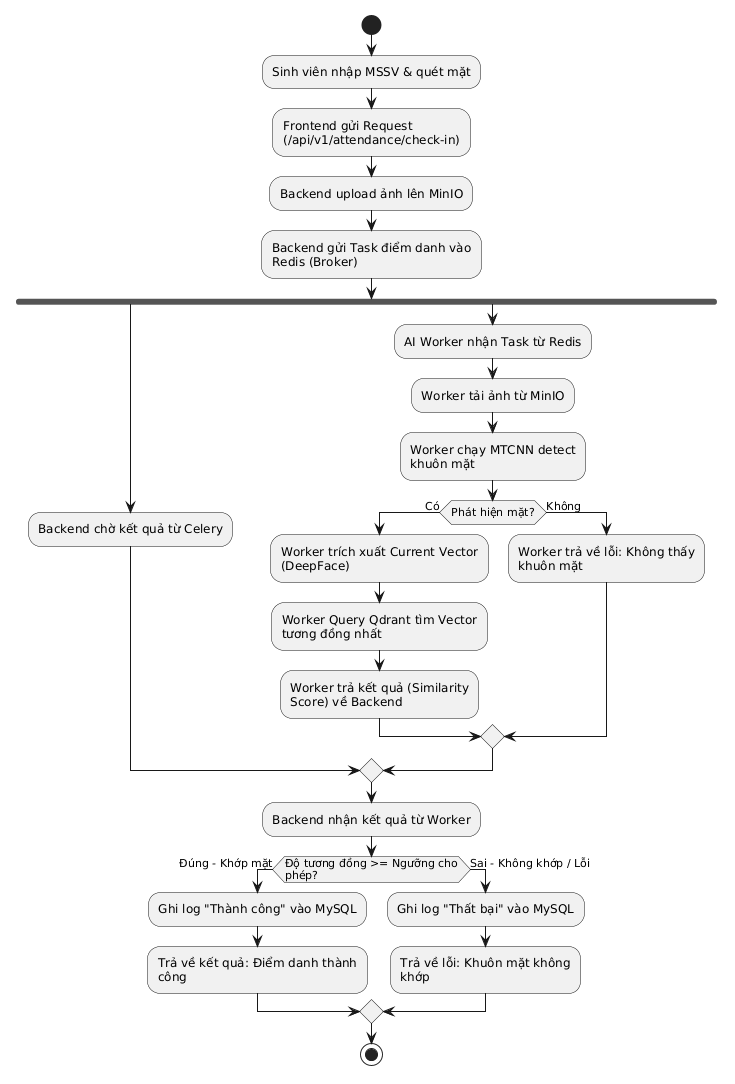
\includegraphics[width=0.85\textwidth,height=0.65\textheight,keepaspectratio]{activity_diem_danh.png}
    \caption{Sơ đồ hoạt động cho luồng điểm danh 1-1}
    \label{fig:activity}
\end{figure}

Hình \ref{fig:activity} thể hiện luồng xác minh 1-1 theo mã sinh viên: nếu không có mã hoặc không tồn tại dữ liệu vector thì trả lỗi sớm; nếu có, worker trích xuất vector, tính độ tương đồng với ngưỡng, trả về kết quả khớp/không khớp.

% =====================================================
% CHƯƠNG 4: USE CASE DIAGRAM
% =====================================================
\chapter{Phân tích Use Case}

\section{Use Case tổng thể}
Sơ đồ Use Case tổng thể (Hình \ref{fig:usecase}) thể hiện toàn bộ chức năng của hệ thống theo ba nhóm tác nhân chính: Sinh viên, Quản lý/Giảng viên, và Hệ thống tự động.

\begin{figure}[H]
    \centering
    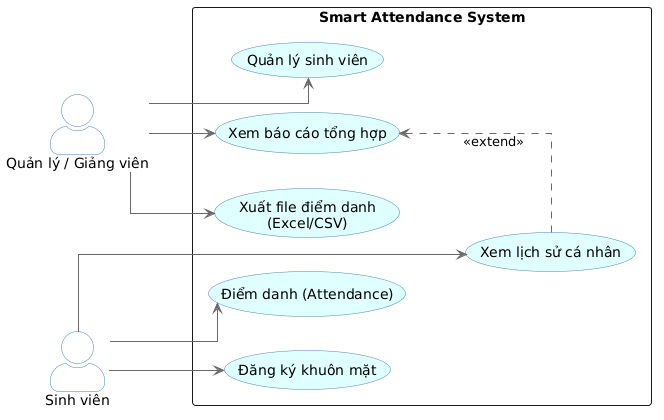
\includegraphics[width=0.95\textwidth]{usecase.png}
    \caption{Sơ đồ Use Case tổng thể hệ thống}
    \label{fig:usecase}
\end{figure}

Hệ thống bao gồm các nhóm chức năng sau:
\begin{itemize}[leftmargin=*]
    \item \textbf{Sinh viên}: Đăng ký khuôn mặt (ảnh/video), đăng ký lịch học, đổi ca học, điểm danh check-in/check-out, xem lịch sử cá nhân.
    \item \textbf{Quản lý/Giảng viên}: Đăng nhập quản trị, duyệt sinh viên, quản lý lịch học (duyệt/từ chối), sửa trạng thái điểm danh, xem dashboard thống kê, xem nhật ký, xuất CSV, xem thông báo.
    \item \textbf{Hệ thống}: Trích xuất vector khuôn mặt (AI), nhận diện khuôn mặt (AI), phát hiện đi muộn, Cronjob quét vắng mặt tự động lúc 23:59.
\end{itemize}

\section{Use Case chi tiết: Đăng ký sinh viên}
Sơ đồ dưới đây (Hình \ref{fig:usecase_dangky}) mô tả chi tiết quy trình đăng ký sinh viên mới, bao gồm đăng ký khuôn mặt (bằng ảnh hoặc video), đăng ký lịch học theo ca, và quy trình xét duyệt bởi giảng viên.

\begin{figure}[H]
    \centering
    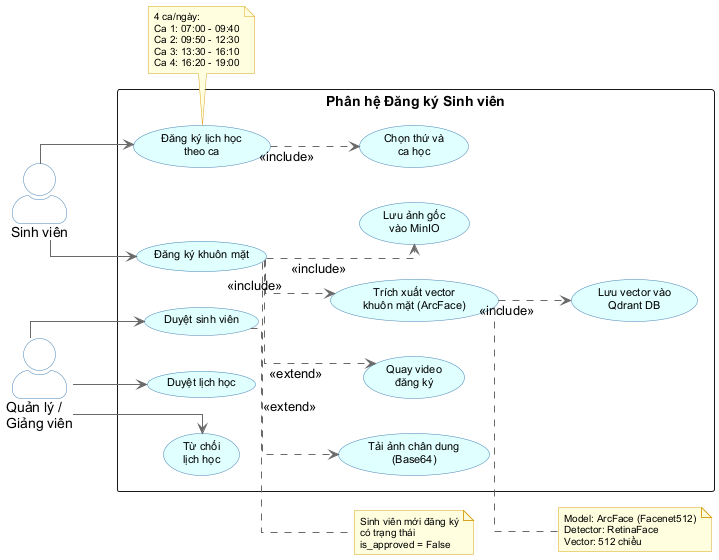
\includegraphics[width=0.95\textwidth]{usecase_dangky.png}
    \caption{Sơ đồ Use Case chi tiết -- Phân hệ Đăng ký sinh viên}
    \label{fig:usecase_dangky}
\end{figure}

\begin{table}[H]
\centering
\begin{tabularx}{\textwidth}{|l|X|}
\hline
\textbf{Use Case} & \textbf{Mô tả} \\ \hline
Đăng ký khuôn mặt & Sinh viên tải ảnh (base64) hoặc quay video. Hệ thống trích xuất vector 512 chiều bằng ArcFace, lưu vào Qdrant và ảnh gốc vào MinIO. \\ \hline
Đăng ký lịch học & Sinh viên chọn thứ và ca học (4 ca/ngày). Lịch ở trạng thái chờ duyệt. \\ \hline
Duyệt sinh viên & Giảng viên duyệt tài khoản mới (is\_approved = True). \\ \hline
Duyệt/Từ chối lịch & Giảng viên phê duyệt hoặc từ chối yêu cầu lịch. Lịch cũ bị vô hiệu hóa khi có lịch mới được duyệt. \\ \hline
\end{tabularx}
\caption{Mô tả Use Case phân hệ Đăng ký}
\end{table}

\section{Use Case chi tiết: Điểm danh}
Sơ đồ dưới đây (Hình \ref{fig:usecase_diemdanh}) mô tả chi tiết quy trình điểm danh đa phiên, bao gồm check-in, check-out, nhận diện khuôn mặt AI, phát hiện đi muộn và xử lý tự động cuối ngày.

\begin{figure}[H]
    \centering
    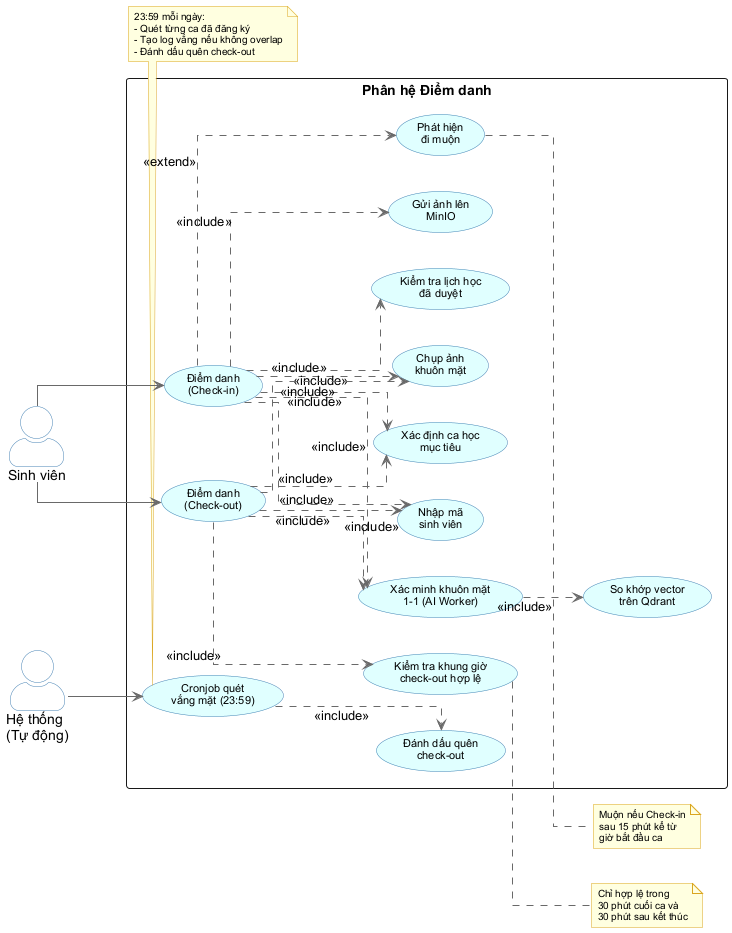
\includegraphics[width=0.95\textwidth]{usecase_diemdanh.png}
    \caption{Sơ đồ Use Case chi tiết -- Phân hệ Điểm danh}
    \label{fig:usecase_diemdanh}
\end{figure}

\begin{table}[H]
\centering
\begin{tabularx}{\textwidth}{|l|X|}
\hline
\textbf{Use Case} & \textbf{Mô tả} \\ \hline
Check-in & Sinh viên nhập MSSV, chụp ảnh. Hệ thống kiểm tra lịch học, gửi ảnh qua Celery Worker xác minh 1-1 với Qdrant. Nếu khớp, ghi log check-in và xác định ca mục tiêu. \\ \hline
Check-out & Tương tự check-in nhưng kiểm tra thêm khung giờ hợp lệ (30 phút cuối ca + 30 phút sau kết thúc). \\ \hline
Phát hiện đi muộn & Tự động đánh dấu nếu check-in sau 15 phút so với giờ bắt đầu ca. \\ \hline
Cronjob quét vắng & Lúc 23:59, quét từng ca đã đăng ký. Tạo log vắng nếu không tìm thấy phiên giao cắt. Đánh dấu quên check-out cho phiên chưa đóng. \\ \hline
\end{tabularx}
\caption{Mô tả Use Case phân hệ Điểm danh}
\end{table}

\section{Use Case chi tiết: Quản trị hệ thống}
Sơ đồ dưới đây (Hình \ref{fig:usecase_quantri}) mô tả chi tiết các chức năng quản trị dành cho giảng viên/admin.

\begin{figure}[H]
    \centering
    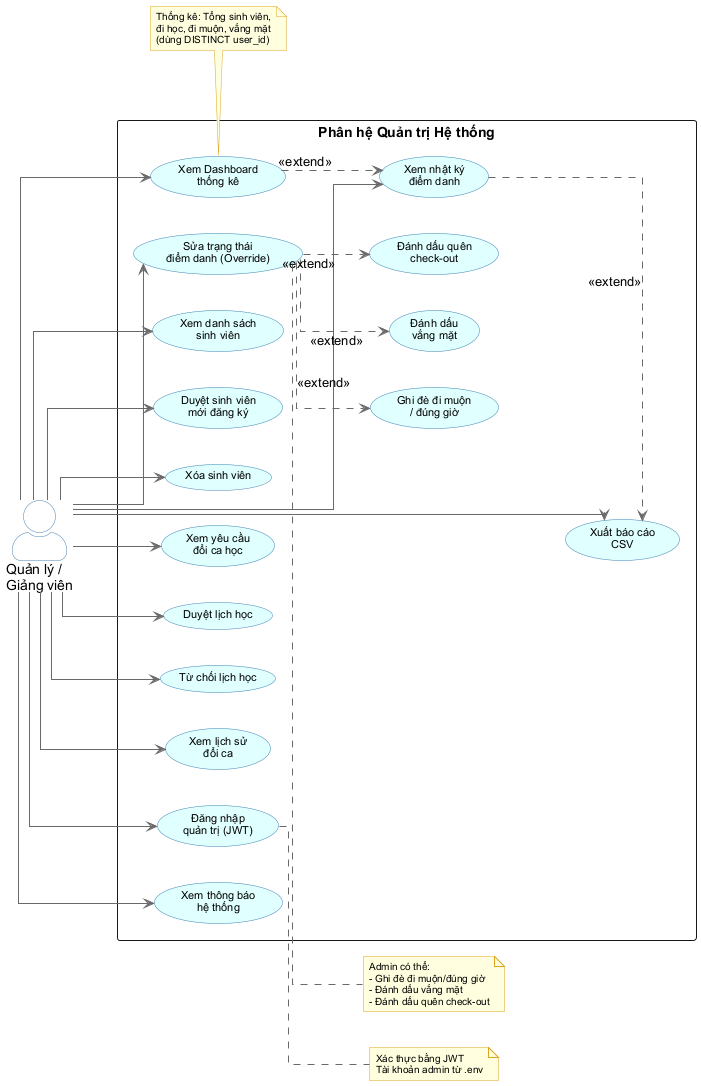
\includegraphics[width=0.95\textwidth]{usecase_quantri.png}
    \caption{Sơ đồ Use Case chi tiết -- Phân hệ Quản trị}
    \label{fig:usecase_quantri}
\end{figure}

\begin{table}[H]
\centering
\begin{tabularx}{\textwidth}{|l|X|}
\hline
\textbf{Use Case} & \textbf{Mô tả} \\ \hline
Đăng nhập quản trị & Xác thực bằng JWT. Tài khoản admin cấu hình từ biến môi trường. \\ \hline
Duyệt/Xóa sinh viên & Phê duyệt tài khoản sinh viên mới hoặc xóa sinh viên khỏi hệ thống. \\ \hline
Quản lý lịch học & Duyệt/từ chối yêu cầu đổi ca. Xem lịch sử đổi ca của sinh viên. \\ \hline
Override điểm danh & Ghi đè trạng thái: đi muộn/đúng giờ, đánh dấu vắng, đánh dấu quên check-out. \\ \hline
Dashboard thống kê & Xem tổng quan: tổng sinh viên, đi học, đi muộn, vắng mặt. \\ \hline
Xuất CSV & Xuất nhật ký điểm danh chi tiết ra file CSV để phục vụ báo cáo. \\ \hline
\end{tabularx}
\caption{Mô tả Use Case phân hệ Quản trị}
\end{table}

% =====================================================
% CHƯƠNG 5: MÀN HÌNH GIAO DIỆN
% =====================================================
\chapter{Màn hình giao diện}

Chương này trình bày các màn hình giao diện chính của hệ thống, minh họa luồng thao tác từ đăng nhập, quản trị đến điểm danh.

\section{Giao diện quản trị (Admin)}

\begin{figure}[H]
    \centering
    \begin{subfigure}[t]{0.48\textwidth}
        \centering
        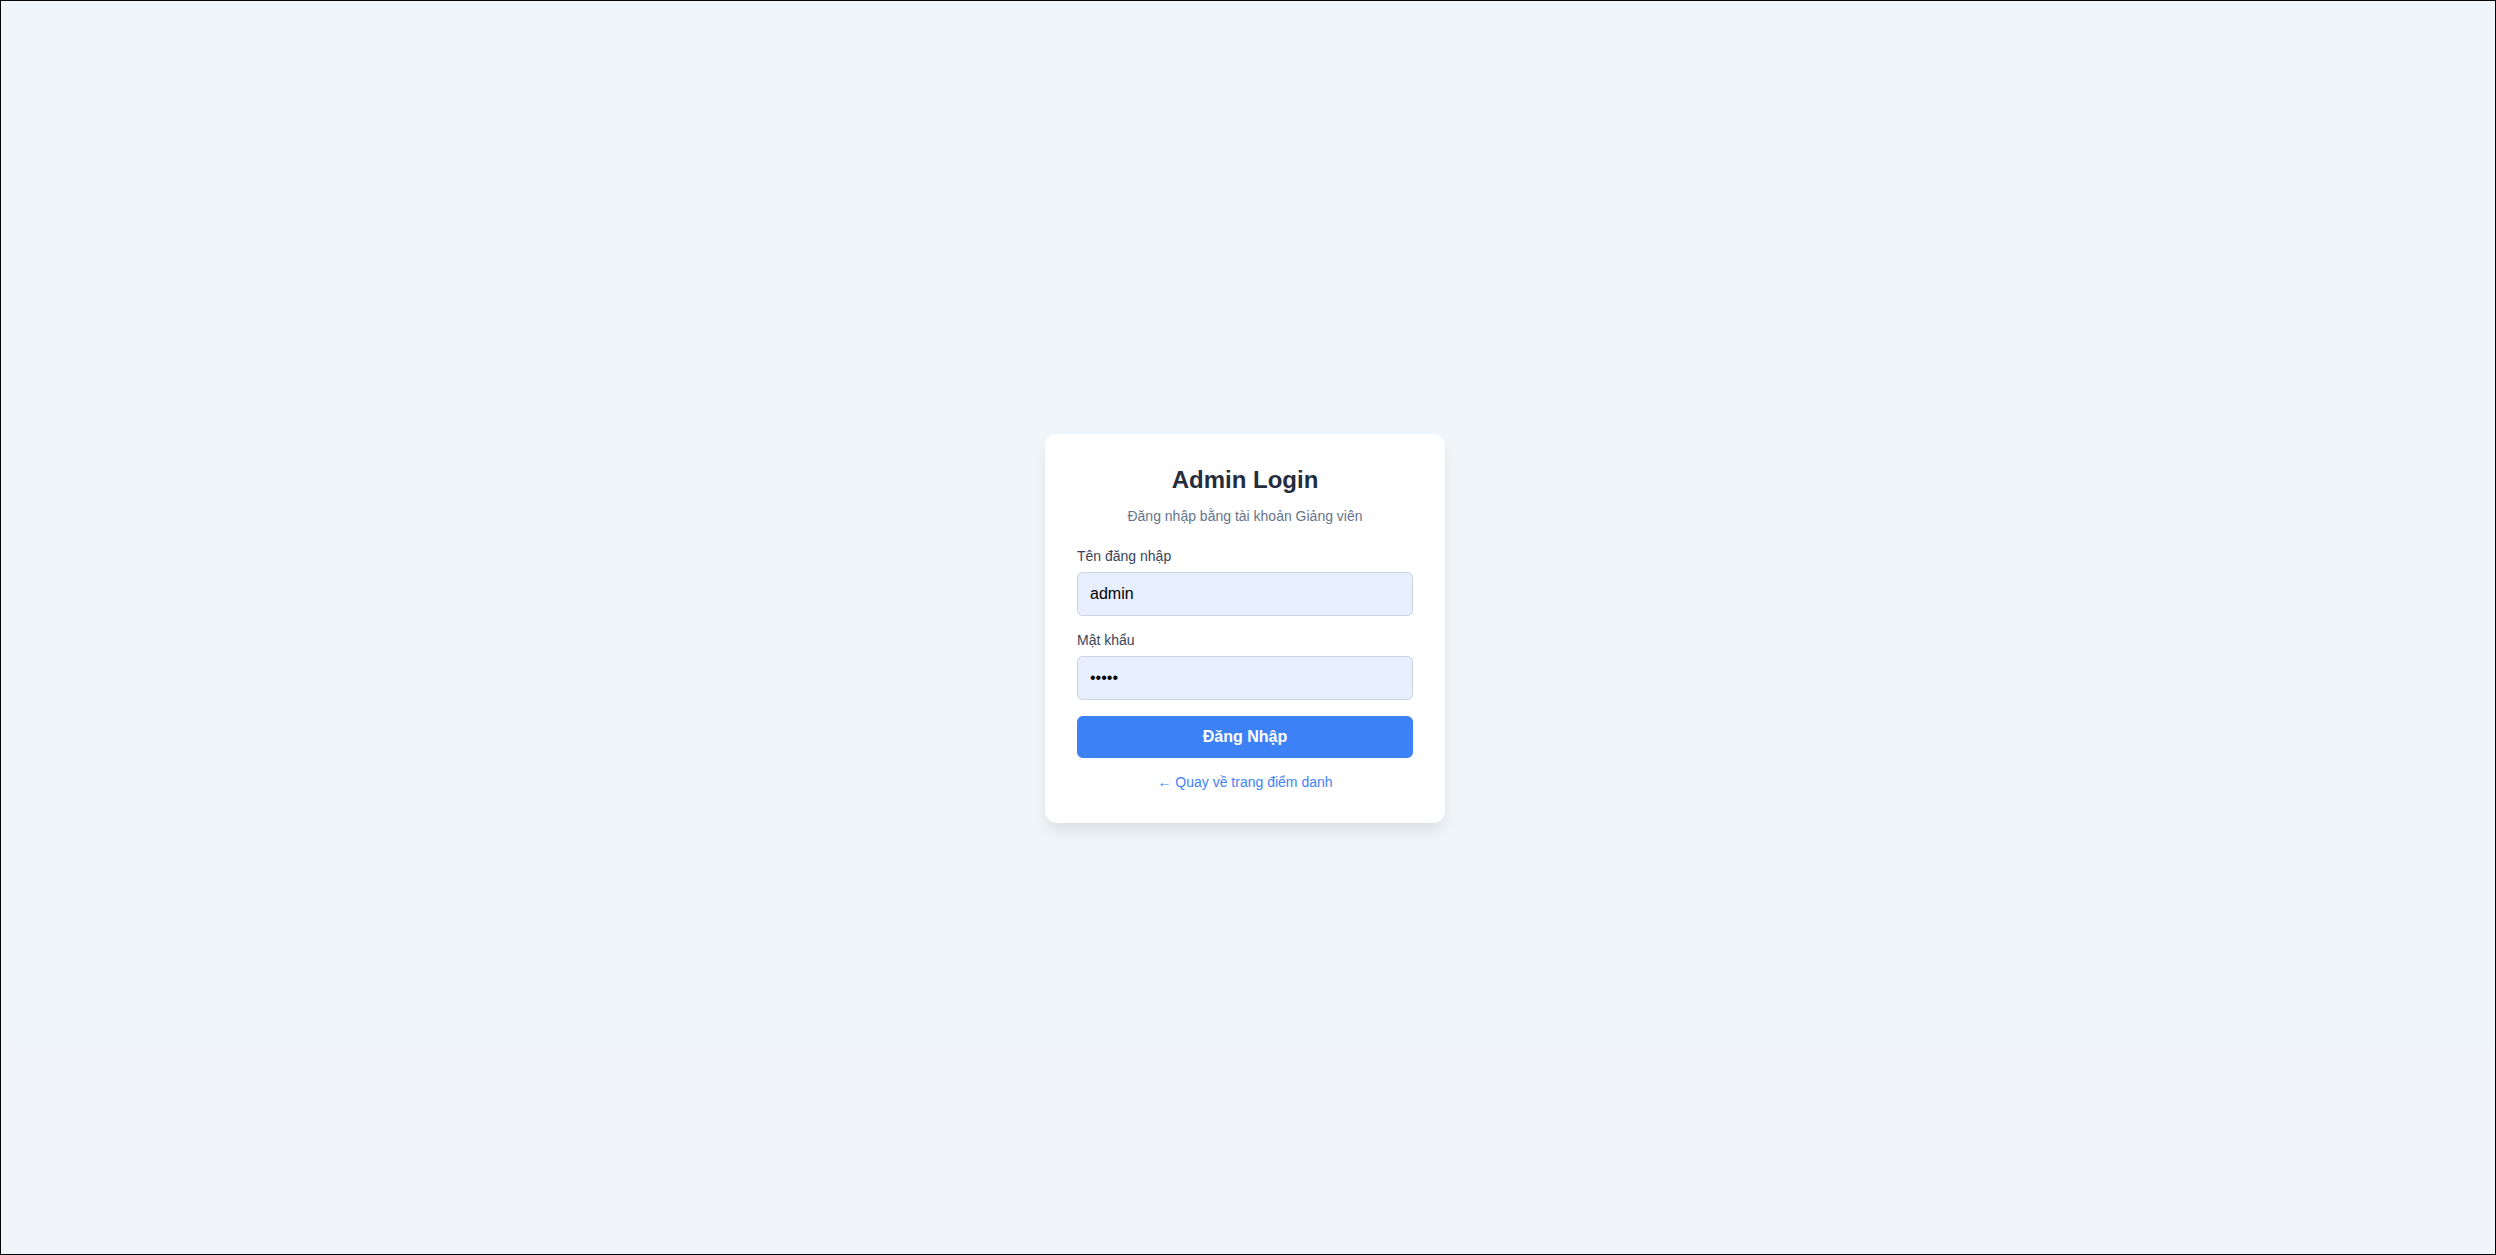
\includegraphics[width=\textwidth]{dang_nhap_admin.png}
        \caption{Đăng nhập Admin}
    \end{subfigure}
    \hfill
    \begin{subfigure}[t]{0.48\textwidth}
        \centering
        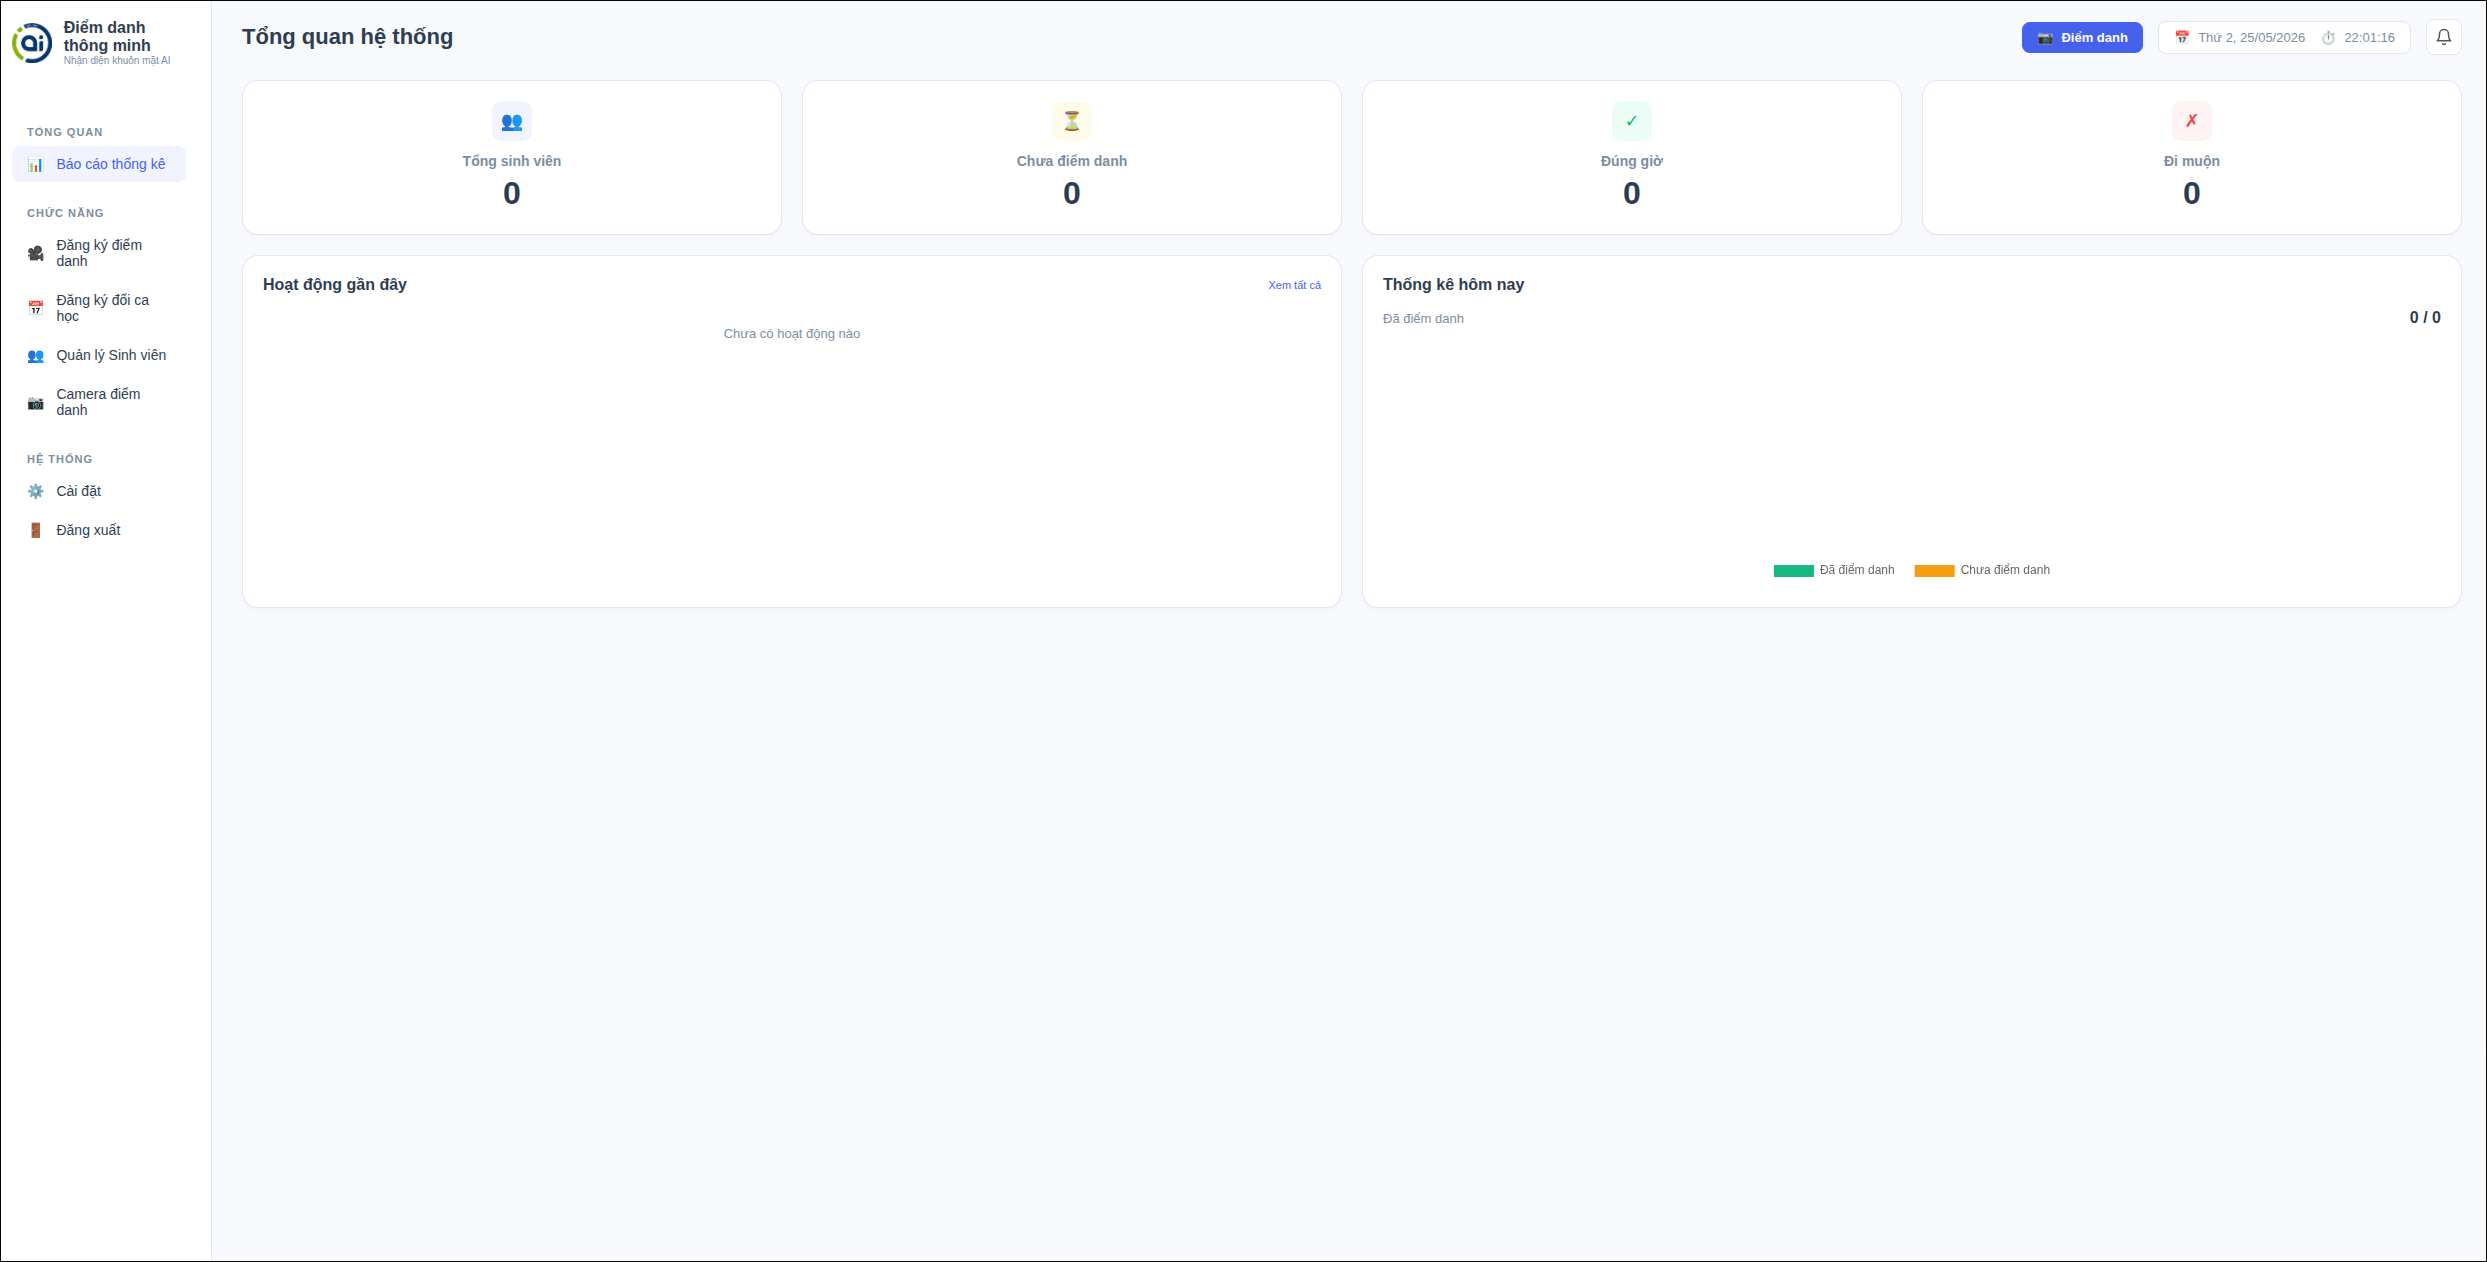
\includegraphics[width=\textwidth]{dashbroad.png}
        \caption{Dashboard thống kê}
    \end{subfigure}
    \caption{Các màn hình quản trị chính của hệ thống}
    \label{fig:demo_admin}
\end{figure}

\textbf{Đăng nhập Admin} (Hình \ref{fig:demo_admin}a): Giảng viên đăng nhập bằng tài khoản quản trị, hệ thống xác thực JWT và chuyển hướng tới dashboard.

\textbf{Dashboard thống kê} (Hình \ref{fig:demo_admin}b): Hiển thị tổng quan số liệu điểm danh trong ngày, bao gồm tổng sinh viên, số người đi học, đi muộn, vắng mặt, cùng biểu đồ trực quan.

\begin{figure}[H]
    \centering
    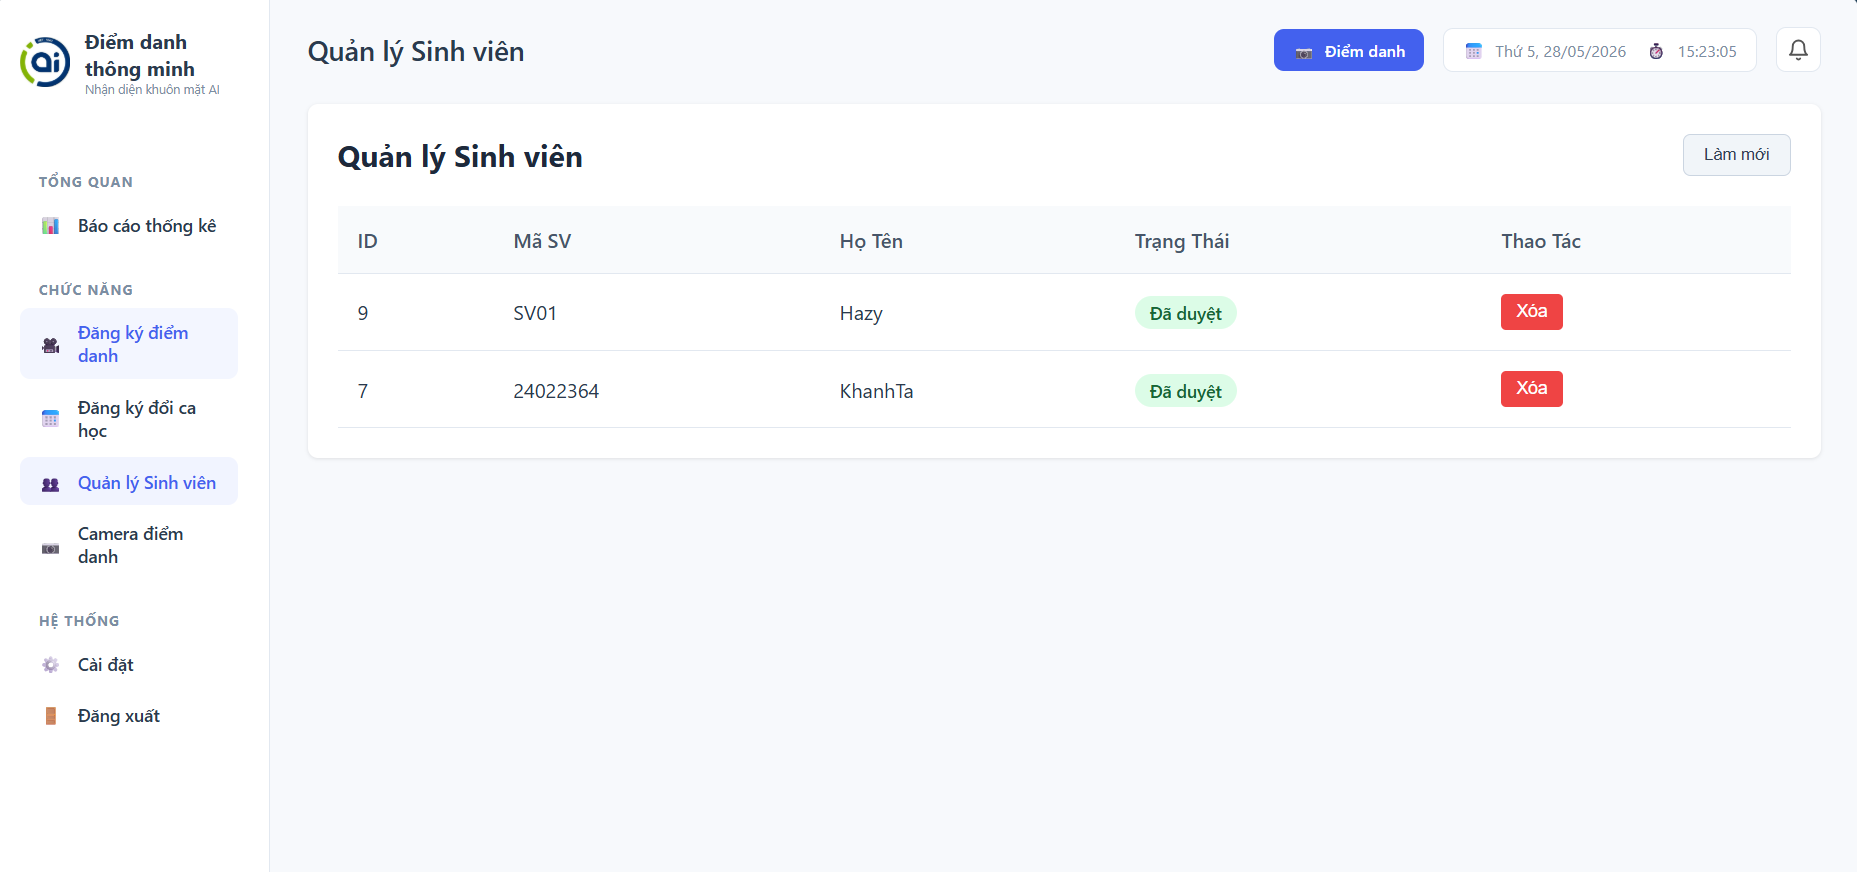
\includegraphics[width=0.8\textwidth]{Admin_QuanLySinhVien.png}
    \caption{Màn hình quản lý sinh viên (Admin)}
    \label{fig:demo_quanlysv}
\end{figure}

\textbf{Quản lý sinh viên} (Hình \ref{fig:demo_quanlysv}): Giao diện danh sách sinh viên cho phép admin duyệt tài khoản mới, xem thông tin chi tiết và xóa sinh viên khỏi hệ thống.

\section{Giao diện sinh viên}

\begin{figure}[H]
    \centering
    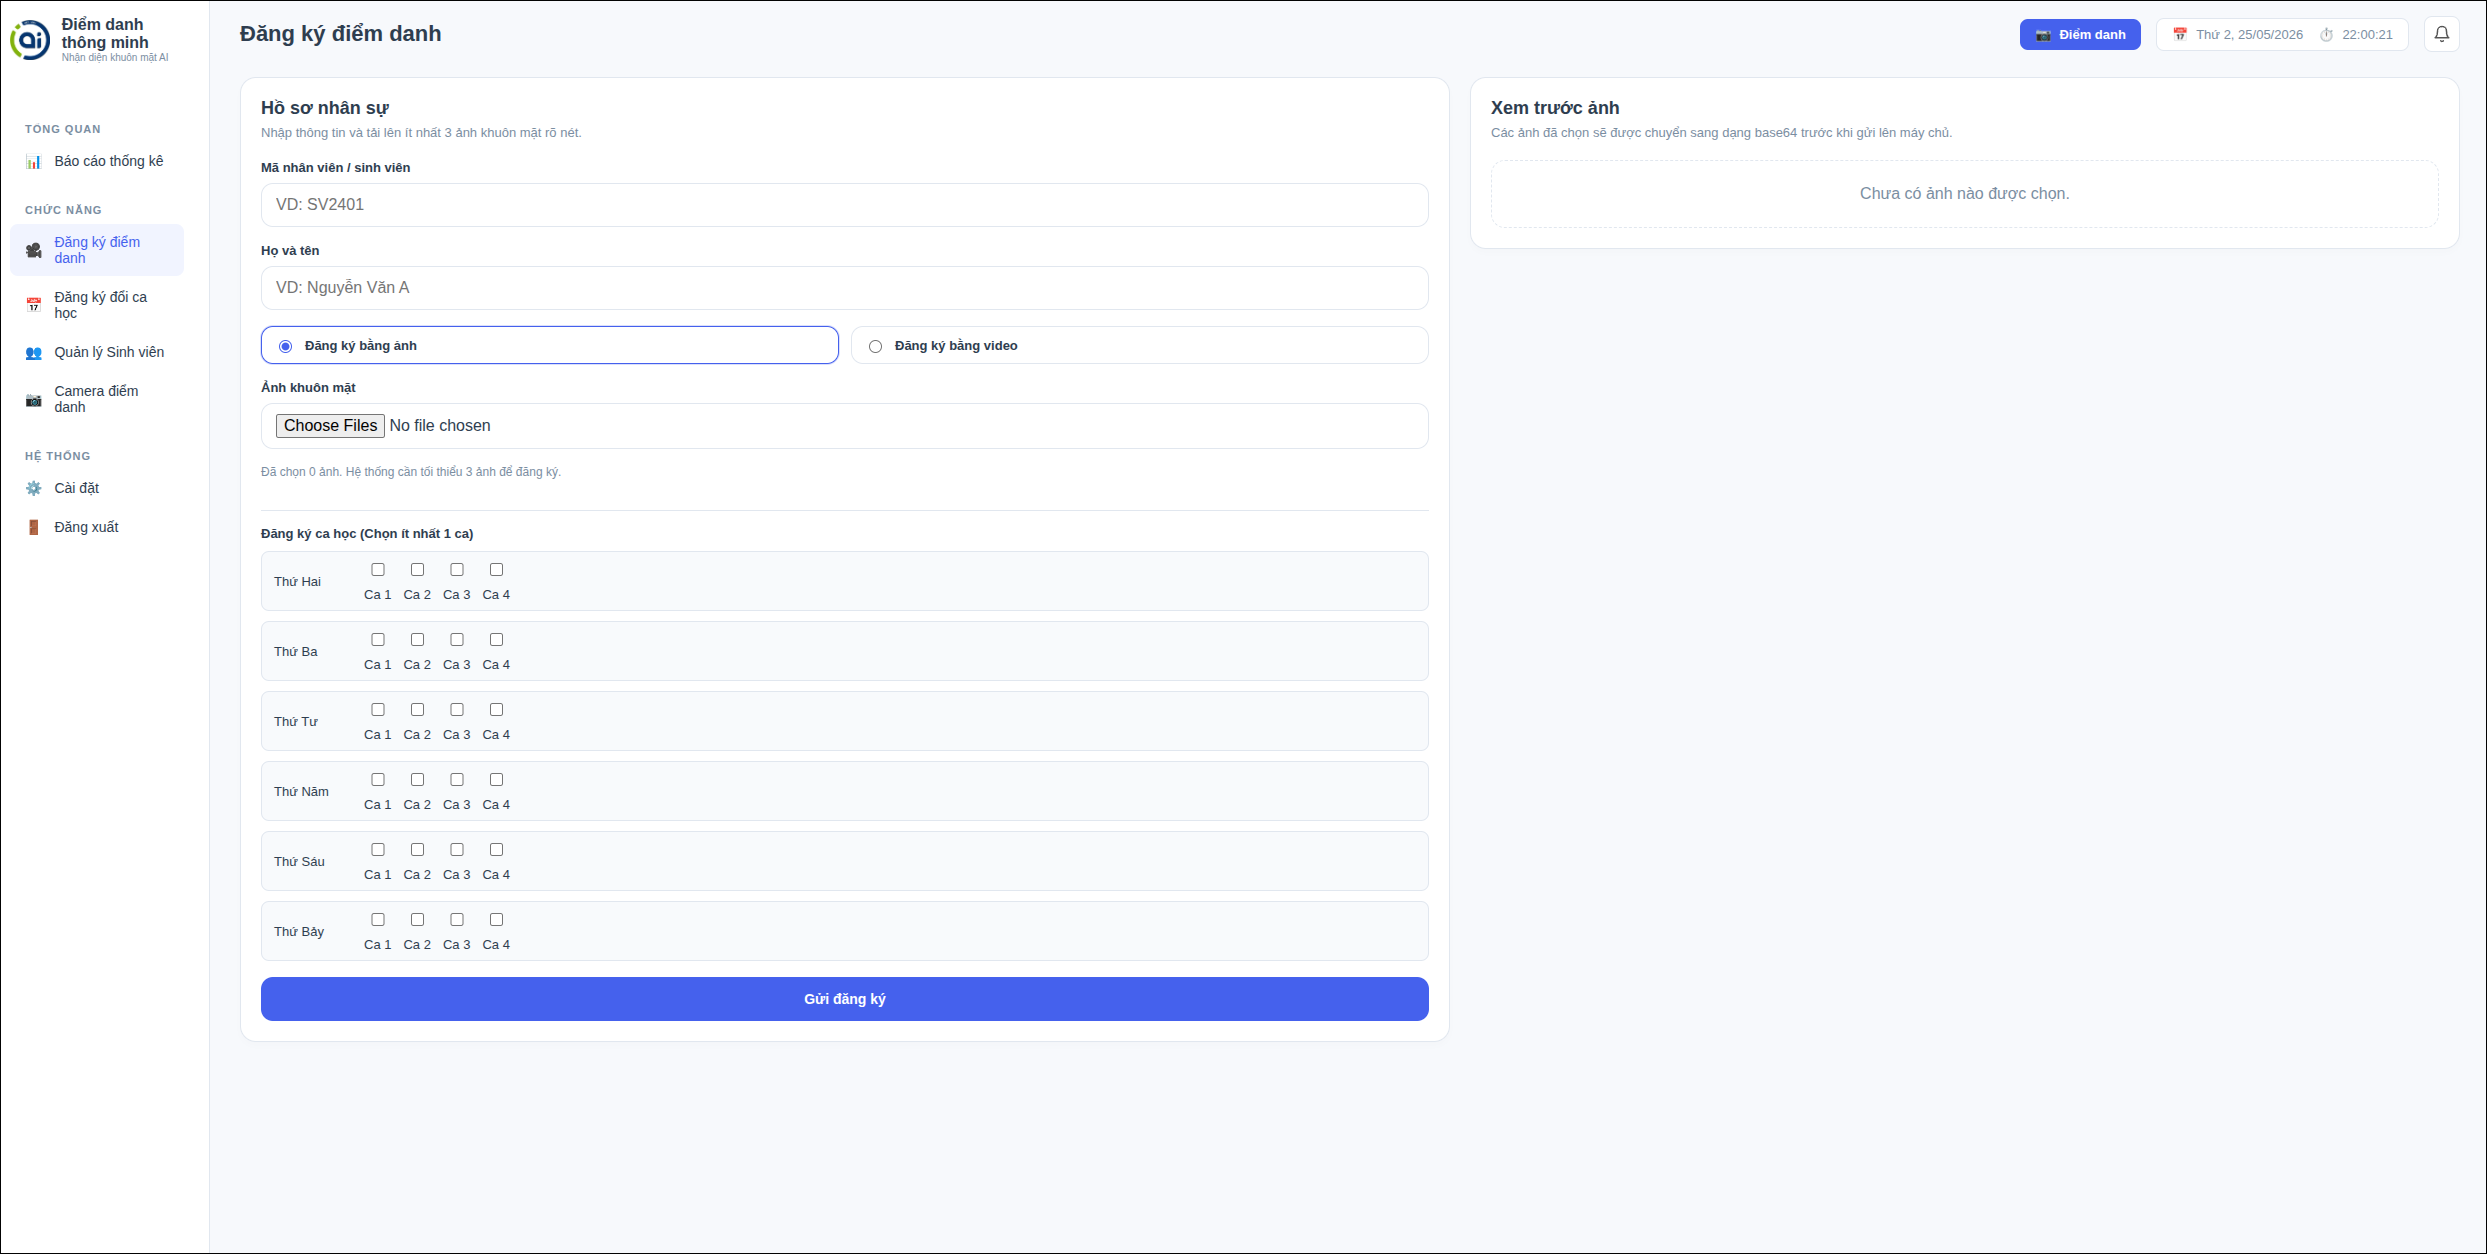
\includegraphics[width=0.7\textwidth]{dang_ki_diem_danh.png}
    \caption{Màn hình đăng ký điểm danh cho sinh viên}
    \label{fig:demo_checkin}
\end{figure}

\textbf{Đăng ký điểm danh} (Hình \ref{fig:demo_checkin}): Sinh viên nhập mã số, chụp ảnh khuôn mặt qua camera hoặc tải ảnh lên. Hệ thống tự động trích xuất vector khuôn mặt và lưu vào cơ sở dữ liệu.

\begin{figure}[H]
    \centering
    \begin{subfigure}[t]{0.48\textwidth}
        \centering
        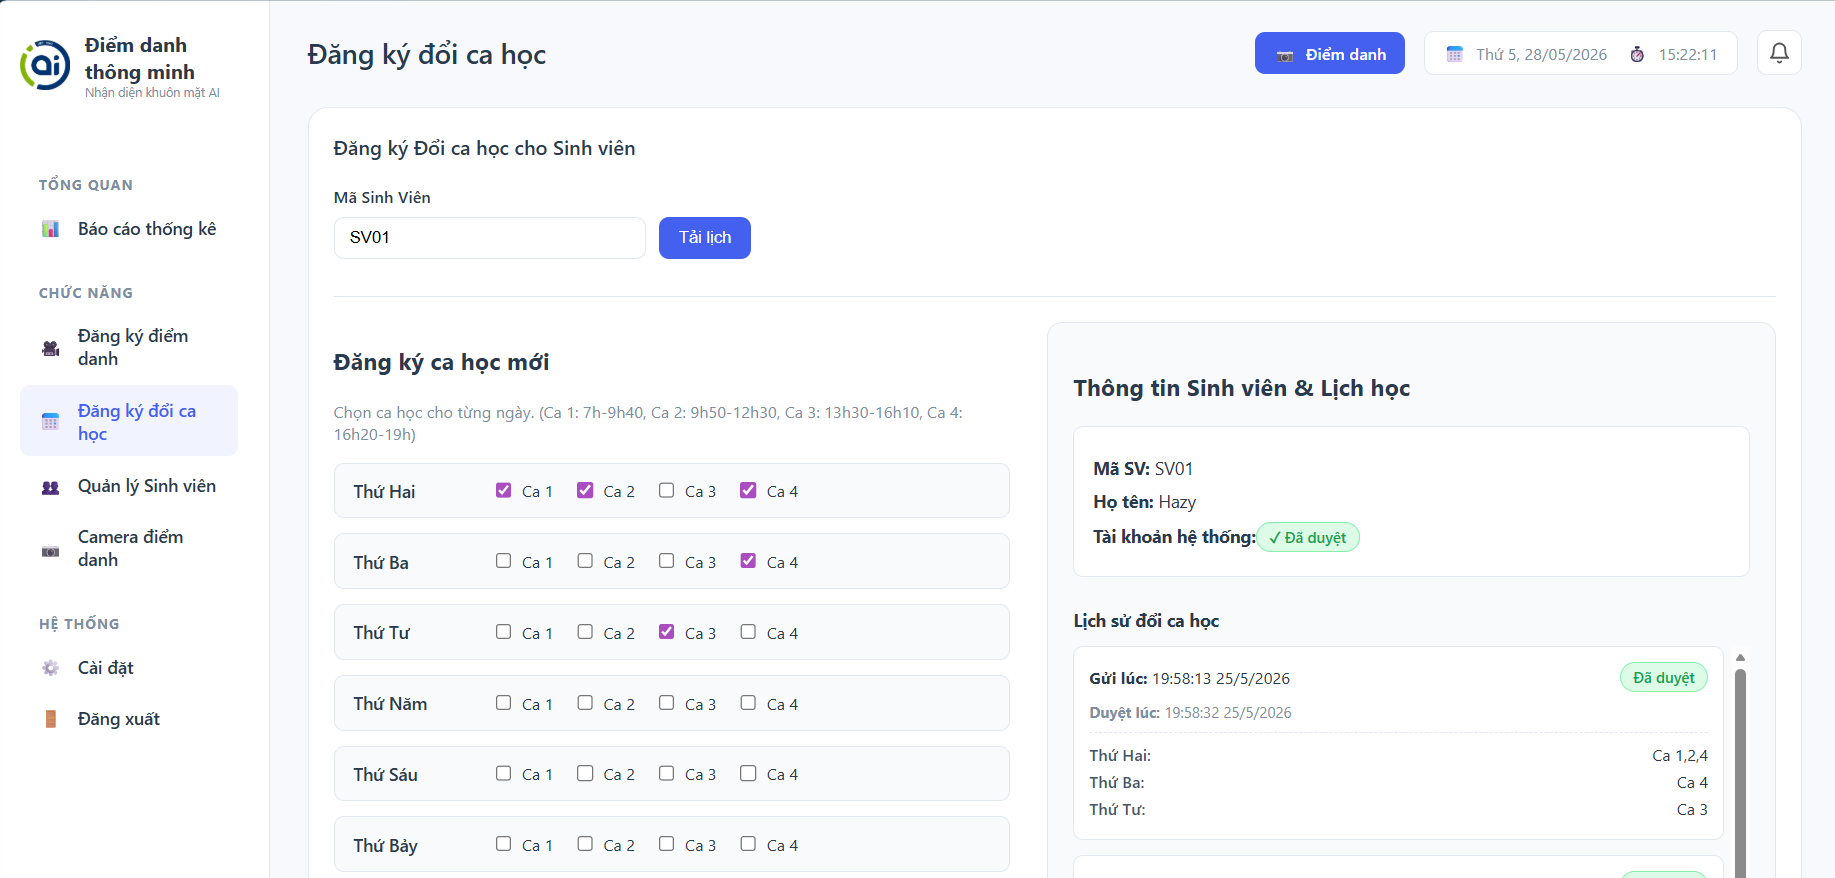
\includegraphics[width=\textwidth]{GiaoDienDoiCaHoc.png}
        \caption{Giao diện đổi ca học}
    \end{subfigure}
    \hfill
    \begin{subfigure}[t]{0.48\textwidth}
        \centering
        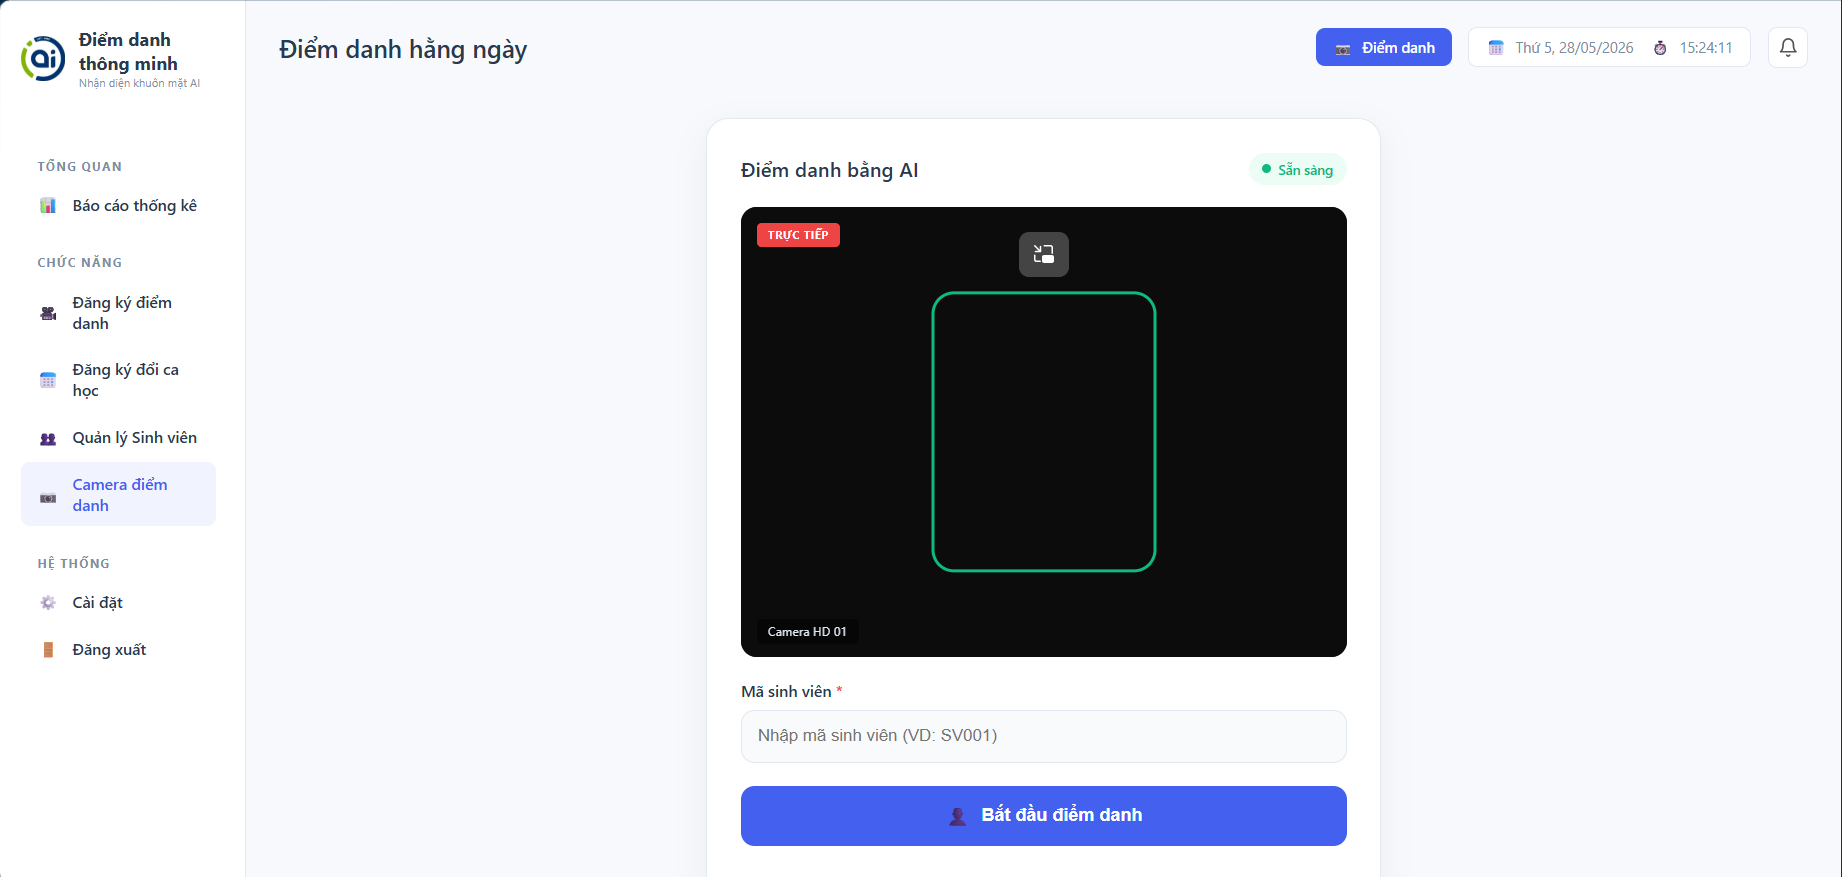
\includegraphics[width=\textwidth]{SV_DiemDanh.png}
        \caption{Giao diện điểm danh sinh viên}
    \end{subfigure}
    \caption{Các màn hình chức năng phía sinh viên}
    \label{fig:demo_sv}
\end{figure}

\textbf{Đổi ca học} (Hình \ref{fig:demo_sv}a): Sinh viên có thể yêu cầu đổi ca học sang ca khác, yêu cầu được gửi về hệ thống chờ giảng viên duyệt.

\textbf{Điểm danh} (Hình \ref{fig:demo_sv}b): Sinh viên nhập MSSV, chụp ảnh khuôn mặt. Hệ thống xác minh 1-1 và ghi nhận trạng thái check-in/check-out theo ca học.

% =====================================================
% CHƯƠNG 6: THIẾT KẾ CƠ SỞ DỮ LIỆU
% =====================================================
\chapter{Thiết kế cơ sở dữ liệu}

\section{Sơ đồ ERD}
\begin{figure}[H]
    \centering
    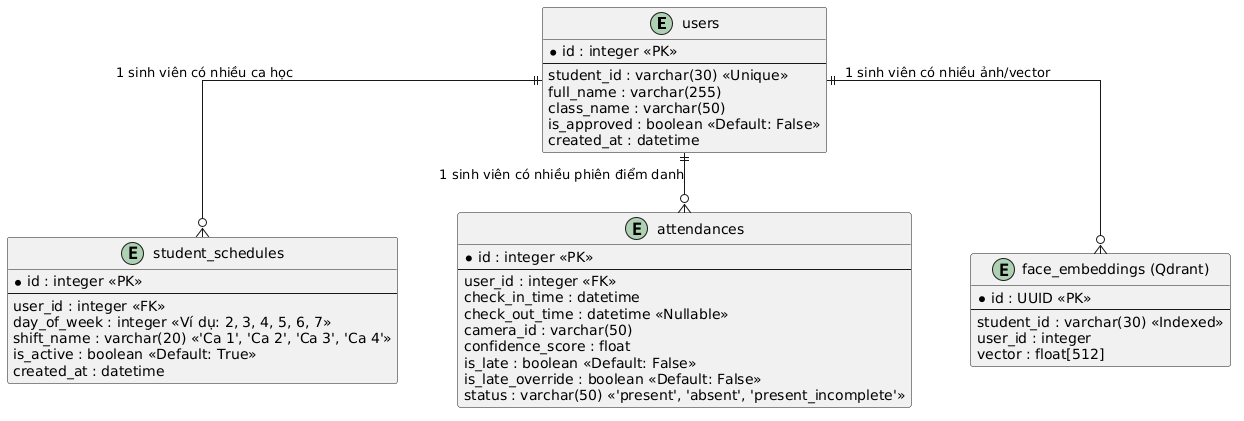
\includegraphics[width=0.8\textwidth]{csdl.png}
    \caption{Sơ đồ ERD cơ sở dữ liệu}
    \label{fig:erd}
\end{figure}

\section{Mô tả các thực thể chính}
\begin{table}[H]
\centering
\begin{tabularx}{\textwidth}{|>{\raggedright\arraybackslash}p{0.45\textwidth}|>{\raggedright\arraybackslash}p{0.50\textwidth}|}
\hline
\textbf{Bảng/Collection} & \textbf{Mô tả} \\ \hline
users & Thông tin sinh viên: MSSV, họ tên, trạng thái duyệt (is\_approved), số ảnh đã đăng ký. \\ \hline
student\_schedules & Lịch học theo ngày/ca, trạng thái duyệt (pending/approved/rejected) và lịch sử đổi ca. \\ \hline
attendances & Log điểm danh chi tiết: loại (check-in/check-out), trạng thái (present/late/absent), thời gian, độ tin cậy. \\ \hline
face\_embeddings (Qdrant) & Vector khuôn mặt 512 chiều lưu trên Qdrant Vector DB, payload chứa student\_id để lọc khi xác minh 1-1. \\ \hline
\end{tabularx}
\caption{Mô tả các thực thể chính}
\end{table}

% =====================================================
% CHƯƠNG 7: TRIỂN KHAI VÀ VẬN HÀNH
% =====================================================
\chapter{Triển khai và vận hành}

\section{Kiến trúc Docker Compose}
Hệ thống đóng gói 8 container độc lập, giao tiếp qua bridge network \texttt{attendance\_net}:

\begin{table}[H]
\centering
\begin{tabularx}{\textwidth}{|l|X|l|}
\hline
\textbf{Service} & \textbf{Chức năng} & \textbf{Cổng} \\ \hline
nginx & Reverse proxy, phục vụ frontend & 8080 \\ \hline
backend & API FastAPI & 8000 (internal) \\ \hline
worker & Celery Worker AI & - \\ \hline
mysql & CSDL quan hệ & 3307 \\ \hline
redis & Queue/Cache & 6379 \\ \hline
qdrant & Vector DB & 6333 \\ \hline
minio & Object Storage & 9000/9001 \\ \hline
backup & Sao lưu định kỳ & - \\ \hline
\end{tabularx}
\caption{Danh sách dịch vụ trong Docker Compose}
\end{table}

\section{Tính năng nâng cao}
\begin{itemize}[leftmargin=*]
    \item \textbf{CI/CD}: Pipeline tự động build và đóng gói Docker image qua GitHub Actions, đảm bảo quy trình phát hành nhất quán.
    \item \textbf{Triển khai Internet}: Hệ thống được public qua domain \code{https://attendance.thanhtech.cloud} với SSL và Nginx gateway.
    \item \textbf{Backup dữ liệu}: Container backup định kỳ dump MySQL, snapshot Qdrant và mirror MinIO, giữ lịch sử 7 ngày.
    \item \textbf{Quản lý cấu hình}: Tham số mô hình AI và ngưỡng nhận diện cấu hình linh hoạt qua file \texttt{.env}.
\end{itemize}

% =====================================================
% CHƯƠNG 8: KẾT LUẬN
% =====================================================
\chapter{Kết luận và hướng phát triển}

\section{Kết luận}
Dự án đã xây dựng thành công một hệ thống điểm danh thông minh với các thành tựu chính:
\begin{itemize}[leftmargin=*]
    \item Xác minh danh tính 1-1 bằng nhận diện khuôn mặt AI (ArcFace + RetinaFace), đạt độ trễ dưới 1.5 giây mỗi lượt điểm danh.
    \item Kiến trúc microservices với 8 container Docker, tách biệt tầng xử lý AI và nghiệp vụ, dễ mở rộng.
    \item Quy trình vận hành đầy đủ: đăng ký, duyệt, điểm danh đa phiên, quét vắng tự động, dashboard thống kê và xuất báo cáo CSV.
    \item Triển khai thực tế trên Internet với SSL, CI/CD tự động và sao lưu định kỳ.
\end{itemize}

\section{Hướng phát triển}
\begin{itemize}[leftmargin=*]
    \item Bổ sung \textit{liveness detection} để chống giả mạo bằng ảnh tĩnh.
    \item Tối ưu scale bằng cách tự động tăng/giảm số lượng worker theo tải.
    \item Nâng cấp dashboard theo dõi thời gian thực bằng WebSocket.
    \item Phát triển ứng dụng mobile để điểm danh tiện lợi hơn.
\end{itemize}

\vspace{1cm}
\begin{center}
\textbf{--- HẾT ---}
\end{center}

\end{document}